\portada

\begin{esquemaExplorador}
  \temaEsquema{Operadores en $\mathcal{C}$}{
    \conceptoEsquema{Matriz adjunta y operadores especiales}{}
    \conceptoEsquema{Operadores hermitianos y unitarios}{}
    \conceptoEsquema{Descomposición espectral}{}
  }
  \temaEsquema{Puertas Cuánticas de Un cúbit}{
    \conceptoEsquema{Matrices de Pauli: X, Y, Z}{}
    \conceptoEsquema{Puerta de Hadamard}{}
    \conceptoEsquema{Puertas de fase: S, T, rotaciones}{}
  }
  \temaEsquema{Geometría en la Esfera de Bloch}{
    \conceptoEsquema{Rotaciones como operadores unitarios}{}
    \conceptoEsquema{Visualización geométrica}{}
    \conceptoEsquema{Generación de puertas arbitrarias}{}
  }
  \temaEsquema{Operadores en $\mathcal{C}^n$}{
    \conceptoEsquema{Sistemas de múltiples cúbits}{}
    \conceptoEsquema{Operadores producto tensorial}{}
    \conceptoEsquema{Operadores no separables}{}
  }
  \temaEsquema{Puertas Cuánticas Controladas}{
    \conceptoEsquema{CNOT y puertas controladas generales}{}
    \conceptoEsquema{Puertas de múltiples controles}{}
    \conceptoEsquema{Universalidad cuántica}{}
  }
  \temaEsquema{Evolución Temporal y Hamiltonianos}{
    \conceptoEsquema{Operadores hermitianos como generadores}{}
    \conceptoEsquema{Matrices exponenciales}{}
    \conceptoEsquema{Simulación de evolución cuántica}{}
  }
\end{esquemaExplorador}

\unirsection{Ideas clave}

\subsection{Introducción y objetivos}

Habiendo establecido la teoría general de operadores lineales en el Tema 3, ahora nos enfocamos en los operadores específicos en $\mathcal{C}$ y $\mathcal{C}^n$ que forman el corazón de la computación cuántica. Estos operadores, cuando satisfacen la condición de unitariedad, se conocen como \textbf{puertas cuánticas} y constituyen los bloques de construcción fundamentales de los algoritmos cuánticos.

Los objetivos específicos de este tema son:

\begin{itemize}
  \item Caracterizar completamente los operadores unitarios y hermitianos en $\mathcal{C}$.
  \item Estudiar las puertas cuánticas fundamentales y su interpretación geométrica.
  \item Analizar cómo los operadores producto tensorial describen sistemas multicúbit.
  \item Desarrollar puertas controladas y entender su implementación.
  \item Conectar operadores hermitianos con la evolución temporal cuántica.
\end{itemize}

\subsection{Operadores lineales en $\mathcal{C}$}

Empecemos con el espacio de un solo cúbit, $\mathcal{C}$. Aquí, los operadores se representan como matrices $2 \times 2$, y su estudio es fundamental para entender la computación cuántica. La dimensión del espacio de matrices $2 \times 2$ es 4, lo que implica que éste es el número de matrices linealmente independientes que cualquier base va a tener.

\begin{eje}
  Las matrices de Pauli $X, Y, Z$ junto con la identidad $I$ es una base.

  Al coincidir el número de matrices del conjunto con la dimensión del espacio, podemos estudiar solo una condición de base, ser linealmente independiente o generar el espacio.

  Veamos que son linealmente independientes. Si existen $a, b, c, d \in \mathcal{C}$ tales que $aI + bX + cY + dZ = 0$, entonces
  \begin{align*}
    0 & = aI + bX + cY + dZ = a\begin{pmatrix} 1 & 0 \\ 0 & 1 \end{pmatrix}+b \begin{pmatrix} 0 & 1 \\ 1 & 0 \end{pmatrix}    +c \begin{pmatrix} 0 & -i \\ i & 0 \end{pmatrix}+d \begin{pmatrix} 1 & 0 \\ 0 & -1 \end{pmatrix} \\
      & = \begin{pmatrix} a+d & b - ic \\ b + ic & a - d \end{pmatrix}\Rightarrow
    \begin{cases}
      a + d = 0  \\
      b - ic = 0 \\
      b + ic = 0 \\
      a - d = 0
    \end{cases} \Rightarrow a = b = c = d = 0\,.
  \end{align*}
\end{eje}

Cualquier matriz hermítica $A = \begin{pmatrix} a & b \\ \overline{b} & c \end{pmatrix}$ con $a, c \in \mathbb{R}$ y $b \in \mathcal{C}$ puede expresarse en esta base de la siguiente manera
$$A = \frac{a+c}{2}I + \Rp(b)X - \Ip(b)Y+ \frac{a-c}{2}Z\,. $$

El postulado 3 de la teoría cuántica establece que la ecuación de Schrödinger para la evolución temporal de un cúbit debe ser un operador unitario.

En cuanto a los operadores unitarios, la condición $U^\dagger U = I$ impone restricciones no lineales sobre los coeficientes de la combinación lineal. Por lo tanto, el conjunto de operadores unitarios no forma un espacio vectorial, sino un grupo bajo la multiplicación de matrices.

\begin{defi}
  Llamaremos \textbf{puertas cuánticas} a los operadores unitarios en $\mathcal{C}^n$.
\end{defi}

\begin{theo}[Parametrización de puertas cuánticas de un cúbit]
  Toda puerta cuántica en $\mathcal{C}$ puede escribirse como
  $$U = \begin{pmatrix} e^{i\alpha} & 0 \\ 0 & e^{i\beta} \end{pmatrix} \begin{pmatrix} \cos\frac{\theta}{2} & \sin\frac{\theta}{2} \\ -\sin\frac{\theta}{2} & \cos\frac{\theta}{2} \end{pmatrix} \begin{pmatrix} e^{-i\alpha} & 0 \\ 0 & e^{-i\beta} \end{pmatrix}\,,$$
  donde $\alpha, \beta, \theta \in \mathbb{R}$.
\end{theo}

\begin{info}
  Debería notarse que esta parametrización no es compatible con el grupo de operadores unitarios $2 \times 2$ isomorfo a $U(2)$ y con dimensión real 4, como cabría esperar. En computación cuántica, típicamente ignoramos fases globales, y es por ello que en realidad estamos trabajando con el grupo $SU(2)/\mathbb{Z}_2 \cong SO(3)$.
\end{info}

\subsection{La esfera de Bloch}
La esfera de Bloch es una representación geométrica de los estados de un cúbit. Cada punto en la superficie de la esfera corresponde a un estado del cúbit.

Todo ket $\ket{a}$ de un cúbit puede ser expresado a partir de dos valores reales, $\theta$ y $\phi$, como:
\[
  \ket{a}=\cos\left(\frac{\theta}{2}\right)\ket{0}+e^{i\phi}\sin\left(\frac{\theta}{2}\right)\ket{1}\ (\theta,\phi)\in [0, \pi]\times[0, 2\pi]
\]

\begin{figure}[H]
  \centering
  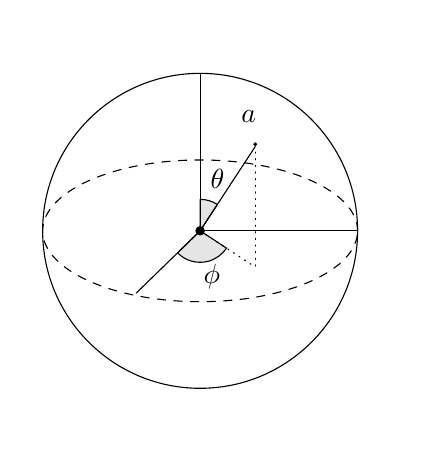
\begin{tikzpicture}
    [line cap=round, line join=round]
    \clip (-2.19,-2.49) rectangle (2.66,2.58);
    \draw [shift={(0,0)}, fill, fill opacity=0.1] (0,0) -- (56.7:0.4) arc (56.7:90.:0.4) -- cycle;
    \draw [shift={(0,0)}, fill, fill opacity=0.1] (0,0) -- (-135.7:0.4) arc (-135.7:-33.2:0.4) -- cycle;
    \draw (0,0) circle (2cm);
    \draw [rotate around={0.:(0.,0.)},dash pattern=on 3pt off 3pt] (0,0) ellipse (2cm and 0.9cm);
    \draw (0,0)-- (0.70,1.07);
    \draw (0,0) -- (0,2);
    \draw (0,0) -- (-0.81,-0.79);
    \draw (0,0) -- (2,0);
    \draw [dotted] (0.7,1) -- (0.7,-0.46);
    \draw [dotted] (0,0) -- (0.7,-0.46);
    \draw (-0.08,-0.3) node[anchor=north west] {$\phi$};
    \draw (0.01,0.9) node[anchor=north west] {$\theta$};
    \draw (0.4,1.65) node[anchor=north west] {$\ket{a}$};
    \scriptsize
    \draw [fill] (0,0) circle (1.5pt);
    \draw [fill] (0.7,1.1) circle (0.5pt);
  \end{tikzpicture}
  \caption{Representación de un ket $\ket{a}\in\H$ en la esfera de Bloch}
\end{figure}

Por convenio, se dibuja la esfera sobre los tres ejes espaciales X, Y, Z de tal modo que el ecuador quede en el plano XY, igualmente se considera el eje Z perpendicular a dicho plano.
Los kets de la base canónica computacional se sitúan sobre el eje Z, estando el ket $\ket{0}$ en el eje positivo y el ket $\ket{1}$ sobre el eje negativo.

\begin{figure}[H]
  \centering
  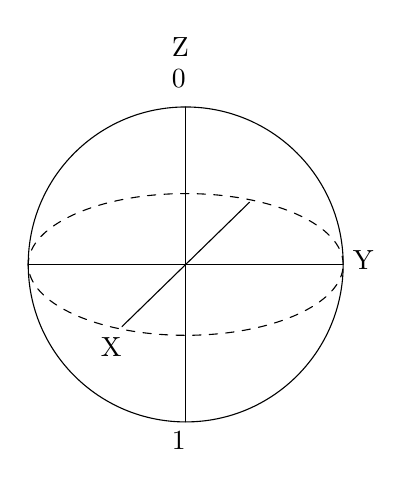
\begin{tikzpicture}
    [line cap=round, line join=round]
    \draw (0,0) circle (2cm);
    \draw [rotate around={0.:(0.,0.)},dash pattern=on 3pt off 3pt] (0,0) ellipse (2cm and 0.9cm);
    \draw (0,0) -- (0,2);
    \draw (0,0) -- (0,-2);
    \draw (0,0) -- (2,0);
    \draw (0,0) -- (-2,0);
    \draw (0,0) -- (-0.81,-0.79);
    \draw (0,0) -- (0.81,0.79);
    \draw (-0.3,3) node[anchor=north west] {Z};
    \draw (-0.3,2.6) node[anchor=north west] {$\ket{0}$};
    \draw (-0.3,-2) node[anchor=north west] {$\ket{1}$};
    \draw (2,0.3) node[anchor=north west] {Y};
    \draw (-1.2,-0.8) node[anchor=north west] {X};
  \end{tikzpicture}
  \caption{Ejes espaciales y representación de la base canónica computacional en la esfera de Bloch}
\end{figure}

\begin{eje}
  Así por ejemplo, el estado $\ket{+} = \frac{1}{\sqrt{2}}(\ket{0} + \ket{1})$ corresponde al punto en el ecuador con $\phi=0$.

  Mientras que $\ket{-} = \frac{1}{\sqrt{2}}(\ket{0} - \ket{1})$ corresponde al punto en el ecuador con $\phi=\pi$.
\end{eje}

\begin{info}
  La esfera de Bloch proporciona una visualización intuitiva de las operaciones cuánticas como rotaciones en el espacio tridimensional. Cada operador unitario en $\mathcal{C}$ corresponde a una rotación de la esfera.
\end{info}

\subsection{Puertas cuánticas fundamentales de un cúbit}

Las matrices de Pauli son las puertas cuánticas más fundamentales y corresponden con rotaciones de $\pi/2$ alrededor de los ejes de la esfera de Bloch. Como puertas dentro del contexto de la computación cuántica, se suelen denotar por las letras $X, Y, Z$, aunque también reciben otros nombres.

\begin{defi}[Puertas de Pauli]
  \begin{align*}
    X & = \begin{pmatrix} 0 & 1 \\ 1 & 0 \end{pmatrix}  & \text{(puerta NOT)}     \\
    Y & = \begin{pmatrix} 0 & -i \\ i & 0 \end{pmatrix}                           \\
    Z & = \begin{pmatrix} 1 & 0 \\ 0 & -1 \end{pmatrix} & \text{(puerta de fase)}
  \end{align*}
\end{defi}

La puerta $X$ a veces se representa como $\oplus$ porque esencialmente es un sumador binario. Para ello solo tenemos que ver como actúa sobre los estados de la base computacional
\begin{align*}
  \ket{0}X & = \ket{1} \quad \text{que es } \ket{0\oplus 1}    \\
  \ket{1}X & = \ket{0} \quad \text{que es } \ket{1\oplus 1}\,,
\end{align*}
donde $\oplus$ es la operación de \textbf{suma binaria}.
Por este motivo, podemos expresar la acción de $X$ sobre la base computacional como
\[
  \ket{a}X = \ket{a\oplus 1}\,,
\]
para $a\in\{0,1\}$.

Para la puerta $Z$ podemos representar su acción sobre la base computacional como
\[
  \ket{a}Z = (-1)^a \ket{a}\,,
\]
para $a\in\{0,1\}$.

\begin{prop}
  La representación de las puertas de Pauli en términos del producto exterior es:
  \begin{enumerate}
    \item $X = \ketbra{0}{1} + \ketbra{1}{0}$.
    \item $Y = i\ketbra{0}{1} - i\ketbra{1}{0}$.
    \item $Z = \ketbra{0}{0} - \ketbra{1}{1}$.
  \end{enumerate}
\end{prop}

Otra puerta comúmente usada es la puerta de Hadamard, que es una puerta cuántica que crea superposiciones equiprobables.

\begin{defi}[Puerta de Hadamard]
  $$H = \frac{1}{\sqrt{2}}\begin{pmatrix} 1 & 1 \\ 1 & -1 \end{pmatrix}$$
\end{defi}

La puerta de Hadamard es fundamental para crear superposiciones, y su acción sobre los estados de la base computacional es:
\begin{itemize}
  \item $\ket{0}H = \frac{1}{\sqrt{2}}(\ket{0} + \ket{1}) = \ket{+}$.
  \item $\ket{1}H = \frac{1}{\sqrt{2}}(\ket{0} - \ket{1}) = \ket{-}$.
\end{itemize}

\begin{defi}[Base de Hadamard]
  Llamaremos base de Hadamard a la base ortonormal $\{\ket{+}, \ket{-}\}$.
\end{defi}
Las siguientes identidades conectan las puertas de Pauli y la puerta de Hadamard:
\begin{align*}
  HXH & = Z  \\
  HZH & = X  \\
  HYH & = -Y
\end{align*}

Para la puerta $H$ podemos representar su acción sobre la base computacional como
\[
  \ket{a}H = \frac{1}{\sqrt{2}}(\ket{0} + (-1)^a \ket{1})\,,
\]
para $a\in\{0,1\}$.

\begin{prop}
  La representación de la puerta de Hadamard en términos del producto exterior es:
  \begin{align*}
    H & = \frac{1}{\sqrt{2}}(\ketbra{0}{0} + \ketbra{1}{1})
  \end{align*}
\end{prop}

Otras puertas más genéricas son las puertas de fase.

\begin{defi}[Puertas de fase]
  \begin{align*}
    R_\phi & = \begin{pmatrix} 1 & 0 \\ 0 & e^{i\phi} \end{pmatrix}  & \text{(puerta de fase general)} \\
    S      & = \begin{pmatrix} 1 & 0 \\ 0 & i \end{pmatrix}          & R_{\frac{\pi}{2}}               \\
    T      & = \begin{pmatrix} 1 & 0 \\ 0 & e^{i\pi/4} \end{pmatrix} & R_{\frac{\pi}{4}}
  \end{align*}
\end{defi}

Las puertas de fase introducen una fase relativa entre los estados $\ket{0}$ y $\ket{1}$, y son cruciales para muchos algoritmos cuánticos. Estas puertas se relacionan entre sí mediante las siguientes identidades:
\begin{itemize}
  \item $S^2 = Z$
  \item $T^2 = S$
  \item $T^4 = Z$
  \item $T^8 = I$
\end{itemize}

\begin{prop}
  La representación de las puertas de fase en términos del producto exterior es:
  \begin{enumerate}
    \item $R_\phi = \ketbra{0}{0} + e^{i\phi}\ketbra{1}{1}$.
    \item $S = \ketbra{0}{0} + i\ketbra{1}{1}$.
    \item $T = \ketbra{0}{0} + e^{i\pi/4}\ketbra{1}{1}$.
  \end{enumerate}
\end{prop}


\subsection{Rotaciones en la Esfera de Bloch}

Toda rotación en la esfera de Bloch corresponde a un operador unitario en $\mathcal{C}$:

\begin{defi}[Rotaciones de Pauli]
  Las rotaciones alrededor de los ejes de Pauli son:
  \begin{align*}
    R_x(\theta) & = e^{-i\theta X/2} = \cos\frac{\theta}{2}I - i\sin\frac{\theta}{2}X = \begin{pmatrix} \cos\frac{\theta}{2} & -i\sin\frac{\theta}{2} \\ -i\sin\frac{\theta}{2} & \cos\frac{\theta}{2} \end{pmatrix} \\
    R_y(\theta) & = e^{-i\theta Y/2} = \cos\frac{\theta}{2}I - i\sin\frac{\theta}{2}Y = \begin{pmatrix} \cos\frac{\theta}{2} & -\sin\frac{\theta}{2} \\ \sin\frac{\theta}{2} & \cos\frac{\theta}{2} \end{pmatrix}    \\
    R_z(\theta) & = e^{-i\theta Z/2} = \cos\frac{\theta}{2}I - i\sin\frac{\theta}{2}Z = \begin{pmatrix} e^{-i\theta/2} & 0 \\ 0 & e^{i\theta/2} \end{pmatrix}
  \end{align*}
\end{defi}

\begin{theo}[Descomposición universal para $SU(2)$]
  Toda matriz unitaria $U \in SU(2)$ puede descomponerse como:
  $$U = e^{i\alpha}R_z(\beta)R_y(\gamma)R_z(\delta)$$
  para algunos ángulos reales $\alpha, \beta, \gamma, \delta$.
\end{theo}

\begin{eje}[Implementación de rotación arbitraria]
  Para implementar una rotación alrededor del vector $\hat{n} = (n_x, n_y, n_z)$ por ángulo $\theta$:
  $$R_{\hat{n}}(\theta) = \cos\frac{\theta}{2}I - i\sin\frac{\theta}{2}(n_xX + n_yY + n_zZ)$$
\end{eje}

\subsection{Operadores en $\mathcal{C}^n$: Sistemas multicúbit}

Recordemos que el espacio de estados de un sistema de $n$ cúbits es el producto tensorial de $n$ copias de $\mathcal{C}$ y tiene dimensión $2^n$, y por construcción de la base computacional, la base canónica de $\mathcal{C}^n$ es
$$\{\ket{b_1 b_2 \ldots b_n} : b_i \in \{0,1\}\}$$

\begin{eje}[Sistema de 2 cúbits]
  Para $n = 2$, tenemos $\mathcal{C}^2$ con base $\{\ket{00}, \ket{01}, \ket{10}, \ket{11}\}$.

  Algunos ejemplo de como actuan las puertas construidas como tensoriales:
  \begin{align*}
    \ket{01}(X \otimes I) & = \ket{0}X \otimes \ket{1}I = \ket{1} \otimes \ket{1} = \ket{11}    \\
    \ket{10}(I \otimes Z) & = \ket{1}I \otimes \ket{0}Z = \ket{1} \otimes \ket{0} = \ket{10}\,.
  \end{align*}
\end{eje}

Sin embargo, no todas las puertas sobre dos cúbits se puede poner como un producto tensorial de dos puertas de un cúbit. Por ejemplo, la puerta CNOT.

\begin{defi}[Puerta CNOT]
  La puerta Controlled-NOT actúa sobre dos cúbits, y se define por
  $$\text{CNOT} = \begin{pmatrix} 1 & 0 & 0 & 0 \\ 0 & 1 & 0 & 0 \\ 0 & 0 & 0 & 1 \\ 0 & 0 & 1 & 0 \end{pmatrix}\,.$$
\end{defi}
La puerta CNOT puede expresarse como suma de productos tensoriales de puertas de un cúbit
$$\text{CNOT} = \ket{0}\bra{0} \otimes I + \ket{1}\bra{1} \otimes X\,.$$
Y como productos externos también se puede expresar como
$$\text{CNOT} = \ketbra{00}{00} + \ketbra{11}{11} + \ketbra{01}{10} + \ketbra{10}{01}\,.$$

\begin{eje}
  \begin{align*}
    \ket{00}\text{CNOT} & = \ket{00} \\
    \ket{01}\text{CNOT} & = \ket{01} \\
    \ket{10}\text{CNOT} & = \ket{11} \\
    \ket{11}\text{CNOT} & = \ket{10}
  \end{align*}
  El nombre de CNOT es Control NOT, pues el primer cúbit actúa como control, esta puerta solo actúa si el primer cúbit está en $\ket{1}$, en tal caso aplica $X$ al segundo cúbit.
\end{eje}

Algunas veces debemos aplicar puertas de un cúbit a sistemas de varios cúbits, y simplemente por el nombre de la puerta no es suficiente para saber dónde actúa la puerta.
Lo habitual es usar el producto tensorial con la unidad para construir nuevas puertas.

\begin{eje}
  La puerta de Hadamard sobre tres cúbits pero actuando solo sobre el segundo se puede construir como $I \otimes H \otimes I$.
\end{eje}

Una notación más compacta y clara es indicar con un subíndice el cúbit sobre el que actúa la puerta.

\begin{eje}
  $H_2$ denota la puerta de Hadamard aplicada al cúbit 2.
  \[
    \ket{001}H_2 = \frac{\ket{001}+\ket{011}}{\sqrt{2}}
  \]
\end{eje}

\subsubsection{Puertas controladas generales}

\begin{defi}[Puerta controlada general]
  Para cualquier operador unitario $U$ de un cúbit:
  $$C_U = \ket{0}\bra{0} \otimes I + \ket{1}\bra{1} \otimes U = \begin{pmatrix} I & 0 \\ 0 & U \end{pmatrix}$$
\end{defi}

\begin{eje}[Otras puertas controladas importantes]
  \begin{itemize}
    \item \textbf{Controlled-Z}: $C_Z = \text{diag}(1, 1, 1, -1)$
    \item \textbf{Controlled-Hadamard}: $C_H = \begin{pmatrix} I & 0 \\ 0 & H \end{pmatrix}$
    \item \textbf{Controlled-Phase}: $C_{R_\phi} = \text{diag}(1, 1, 1, e^{i\phi})$
  \end{itemize}
\end{eje}

Para puertas controladas de dos cúbits, a veces se ejecuta el control sobre el segundo cúbit, pero en estas situaciones, no podemos identificar claramente el control y el objetivo solo por el nombre de la puerta.

En estas situaciones es necesario indicar donde está el cúbit de control.
\begin{defi}
  Sea $U$ una puerta cuántica de un cúbit. Denotamos por $U^j_k$ a la puerta controlada de $U$ con el cúbit $j$ como control y el cúbit $k$ como objetivo.
\end{defi}

\begin{eje}
  \begin{itemize}
    \item La puerta controlada CNOT se puede escribir como $X^1_2$.
    \item La puerta controlada Hadamard se puede escribir como $H^1_2$.
    \item La puerta controlada $X^2_1$ esta representada por la matriz
          $$\begin{pmatrix} 1 & 0 & 0 & 0 \\ 0 & 0 & 0 & 1 \\ 0 & 0 & 1 & 0 \\ 0 & 1 & 0 & 0 \end{pmatrix}\,.$$
  \end{itemize}
\end{eje}

\begin{prop}
  Se dan las siguientes igualdades:
  \begin{align*}
    X^2_1 & = (H\otimes H)X^1_2 (H\otimes H)\,. \\
    Z^2_1 & = Z^1_2\,.                          \\
    X^1_2 & = H_1Z^1_2 H_2\,.
  \end{align*}
\end{prop}

\subsubsection{Puerta SWAP}
\begin{defi}
  La puerta SWAP intercambia dos cúbits
  $$\text{SWAP} = \begin{pmatrix} 1 & 0 & 0 & 0 \\ 0 & 0 & 1 & 0 \\ 0 & 1 & 0 & 0 \\ 0 & 0 & 0 & 1 \end{pmatrix}\,.$$
\end{defi}

\begin{prop}
  La puerta SWAP cumple
  \[
    \text{SWAP} = X^2_1 X^1_2 X^2_1\,.
  \]
\end{prop}

\subsubsection{Puertas de múltiples controles}

\begin{defi}
  Sea $U$ una puerta cuántica de un cúbit. Denotamos por $U^{j_1 j_2 \ldots j_m}_k$ a la puerta controlada de $U$ con el cúbit $j_1, j_2, \ldots, j_m$ como control y el cúbit $k$ como objetivo.
\end{defi}

\begin{defi}[Puerta Toffoli (CCNOT)]
  La puerta Toffoli es un CNOT con dos controles
  $$\text{CCNOT} = X^{12}_3 = \begin{pmatrix} 1 & 0 & 0 & 0 & 0 & 0 & 0 & 0 \\ 0 & 1 & 0 & 0 & 0 & 0 & 0 & 0 \\ 0 & 0 & 1 & 0 & 0 & 0 & 0 & 0 \\ 0 & 0 & 0 & 1 & 0 & 0 & 0 & 0 \\ 0 & 0 & 0 & 0 & 1 & 0 & 0 & 0 \\ 0 & 0 & 0 & 0 & 0 & 1 & 0 & 0 \\ 0 & 0 & 0 & 0 & 0 & 0 & 0 & 1 \\ 0 & 0 & 0 & 0 & 0 & 0 & 1 & 0 \end{pmatrix}\,.$$

  Aplica $X$ al tercer cúbit solo si los primeros dos están en $\ket{11}$.
\end{defi}

\subsection{Evolución Temporal y Hamiltonianos}

Recordemos que la evolución temporal de un sistema cuántico aislado está gobernada por la ecuación de Schrödinger estacionaria
$$\frac{d}{dt}\ket{\psi(t)} = -\frac{i}{\hbar}H\ket{\psi(t)}\,,$$
donde $H$ es el Hamiltoniano (operador hermitiano).

La solución formal es:
$$\ket{\psi(t)} = e^{-iHt/\hbar}\ket{\psi(0)}$$

\begin{eje}[Evolución bajo Hamiltoniano de Pauli]
  Para $H = \omega Z/2$ tenemos que
  $$e^{-iHt} = e^{-i\omega t Z/2} = \cos\frac{\omega t}{2}I - i\sin\frac{\omega t}{2}Z = \begin{pmatrix} e^{-i\omega t/2} & 0 \\ 0 & e^{i\omega t/2} \end{pmatrix}\,.$$

  Un cúbit inicialmente en $\ket{+}$ evoluciona como
  $$\ket{\psi(t)} = \frac{1}{\sqrt{2}}(e^{-i\omega t/2}\ket{0} + e^{i\omega t/2}\ket{1})\,.$$
\end{eje}

Como sabemos calcular la exponencial de una matriz a partir de sus valores propios y vectores propios, podemos calcular la exponencial de un Hamiltoniano.

Para una matriz hermitiana $H$ con descomposición espectral $H = \sum_i \lambda_i P_i$ donde $P_i$ son las proyecciones sobre los subespacios propios, tenemos que
$$e^{-iHt} = \sum_i e^{-i\lambda_i t} P_i\,.$$

\begin{eje}[Exponencial de combinaciones de Pauli]
  Para $H = \alpha X + \beta Y + \gamma Z$ con $|\vec{n}| = \sqrt{\alpha^2 + \beta^2 + \gamma^2}$,
  $$e^{-iHt} = \cos(|\vec{n}|t)I - i\sin(|\vec{n}|t)\frac{\vec{n} \cdot \vec{\sigma}}{|\vec{n}|}\,.$$
\end{eje}

\begin{theo}
  Cualquier operador unitario en $\mathcal{C}^n$ puede aproximarse arbitrariamente bien usando solo las puertas $H$, $T$, y CNOT.
\end{theo}

\begin{info}
  Este resultado es fundamental para la computación cuántica práctica, ya que muestra que solo necesitamos implementar físicamente un pequeño conjunto de puertas para realizar cualquier cálculo cuántico.
\end{info}

\begin{eje}[Estados de Bell]
  A partir del estádo básico $\ket{00}$ podemos construir cualquier estado de Bell aplicando las puertas $H$ y $X^1_2$. Por ejemplo
  \[
    \ket{00}H_1 X^1_2 = \frac{1}{\sqrt{2}}(\ket{00} + \ket{10})X^1_2 = \frac{1}{\sqrt{2}}(\ket{00} + \ket{11}) = \ket{\Phi^+}\,.
  \]
\end{eje}

\begin{eje}[Estado GHZ]
  El estado Greenberger-Horne-Zeilinger (GHZ) es un estado de tres cúbits que es un estado de Bell generalizado. Su construcción es similar a la de los estados de Bell, pero en lugar de aplicar $X^1_2$ aplicamos $X^1_2 X^2_3$.
  \[
    \ket{000}H_1 X^1_2 X^2_3 = \frac{1}{\sqrt{2}}(\ket{000} + \ket{111}) = \ket{\text{GHZ}}\,.
  \]
\end{eje}

Por último veamos el teorema de no clonación. Este teorema nos impide clonar estados cuánticos arbitrariamente y es el motivo por el que no podemos implementar clonadores cuánticos o dicho de otra manera, no podemos hacer copias de estados cuánticos.

\begin{theo}[Teorema de no clonación]
  No existe un operador unitario que pueda clonar estados cuánticos arbitrariamente.
\end{theo}
